\documentclass[a4paper, 10pt]{article}
\usepackage[utf8]{inputenc}
\usepackage[T1]{fontenc}
\usepackage{lmodern}
\usepackage{graphicx}
\usepackage{amsmath}
\usepackage{amssymb}
\usepackage{booktabs}
\usepackage{url}
\usepackage{multirow}
\usepackage{authblk} % Hỗ trợ định dạng tác giả/địa chỉ đa cấp
\usepackage[margin=2.5cm]{geometry} % Thiết lập margin
\usepackage[hidelinks]{hyperref} % Tạo siêu liên kết, KHÔNG CÓ VIỀN ĐỎ
\usepackage{tabularx} % Gói để chỉnh sửa bảng (dùng cột X)
\usepackage{caption} % Xử lý chú thích hình ảnh/bảng

% THIẾT LẬP BIBLATEX
\usepackage[style=numeric-comp, sorting=none, backend=biber]{biblatex}
\addbibresource{references.bib} % Đảm bảo file này tồn tại trong cùng thư mục
% Định nghĩa tiêu đề và tác giả
\title{\textbf{Bluetooth-Controlled 8x32 LED Matrix}}
% CÁCH KHAI BÁO TÁC GIẢ TỐI GIẢN VÀ ÍT LỖI NHẤT
\author[1]{Pham Tuan Anh}
\author[1]{Le Tuan Kiet}
\author[1]{Truong Thao Vi}
\author[1]{Dang Hong Phuoc} 
% Khối địa chỉ cơ quan
\affil[1]{\small FPT University Ho Chi Minh Campus, Vietnam, Lot E2a-7, D1 Street, Saigon Hi-Tech Park, Tang Nhon Phu Ward, HCMC}
% Khối email (Đã gỡ lệnh \\ để tránh lỗi \crcr trong affil)
\affil{
	\vspace{0.3cm}
	\texttt{\small anhtph911@gmail.com, lekiet2442005@gmail.com} \\
	\texttt{\small thaovicotntctv@gmail.com, dangp2660@gmail.com}
}
\date{} % <--- LỆNH QUAN TRỌNG ĐỂ ẨN NGÀY THÁNG NĂM
\begin{document}
	
	\maketitle % Tạo tiêu đề và tên tác giả/địa chỉ
	
	% --- Abstract ---
	\begin{abstract}
		The Bluetooth-Controlled 8x32 LED Matrix project functions as a sophisticated Personal Ambient Notifier, providing a dynamic, real-time information display controlled wirelessly via a smartphone. At its core, the system utilizes an Arduino microcontroller to act as the central processing unit, integrating data from several key components. It ensures continuous environmental awareness through a DS1307 RTC (Real-Time Clock) for accurate time and date tracking, and an LM35 analog sensor for precise ambient temperature measurement. Wireless interactivity is achieved via an HC-05 Bluetooth module, enabling bi-directional data transfer for real-time remote updates of personal messages. The 8x32 LED matrix serves as the primary visual output, displaying time, temperature, and custom text efficiently, while EEPROM (Electrically Erasable Programmable Read-Only Memory) provides non-volatile storage for preserving settings and user messages even when power is off. This specialized architecture enables users to seamlessly manage and update content, positioning the project as an ideal, non-intrusive solution for personal smart environments and modern workspaces.
	\end{abstract}
	
	% --- Mục lục ---
	\newpage
	\tableofcontents
	\newpage
	
	% --- Introduction ---
	\section{Introduction}
	The rapid growth of the Internet of Things (IoT) and smart devices has fueled an increasing demand for flexible and non-intrusive information displays in personal environments. Traditional methods of receiving notifications, often relying on smartphone alerts or static physical notes, can be disruptive or quickly outdated. This context highlights the need for dedicated, ambient devices that offer relevant information without demanding constant attention.
	This project addresses this requirement by developing the Personal Ambient Notifier (Bluetooth-Controlled 8x32 LED Matrix). The system offers a refined solution to personal data management by integrating essential functionalities: precise real-time clock tracking (via DS1307 RTC) and continuous ambient temperature monitoring (via LM35 sensor). Most importantly, the system leverages the HC-05 Bluetooth module to enable seamless wireless communication, allowing users to remotely transmit and update personalized text messages to the 8x32 LED matrix display from a standard smartphone.
	By utilizing the robust Arduino microcontroller as the central hub and EEPROM for non-volatile storage, this project delivers a highly functional, low-cost platform. It successfully merges the utility of a digital timepiece, an environmental sensor, and a dynamic communication board into a single, aesthetically pleasing device, making it an ideal component for any modern workspace or personal smart environment.
	
	% --- Main Proposal ---
	\section{Main Proposal}
	
	\subsection{System models and block diagram}
	The Personal Ambient Notifier system is designed based on a robust, modular architecture, ensuring clarity in data acquisition, processing, and output. Fig.~\ref{fig:block_diagram} illustrates the core components and the principal data flow.
	
	\subsubsection{Data Flow and Component Roles}
	\begin{itemize}
		\item \textbf{Input \& Data Acquisition:} This stage involves collecting the necessary environmental data and external commands.
		\begin{itemize}
			\item \textit{External Command:} A Smartphone running a Bluetooth controller application sends custom text messages and commands wirelessly to the \textbf{Bluetooth Module (HC-05)}.
			\item \textit{Time Data:} The \textbf{Real-Time Clock Module (DS1307 RTC)} supplies continuous, accurate time and date data.
			\item \textit{Environmental Data:} The \textbf{Temperature Sensor (LM35)} measures and provides the ambient temperature reading.
		\end{itemize}
		\item \textbf{Processing Unit:} The \textbf{Arduino microcontroller} acts as the central hub, receiving, prioritizing, and processing data.
		\item \textbf{Output \& Display:} The \textbf{LED Matrix (8x32)} serves as the final visual output device, displaying time, temperature, and custom messages with dynamic scrolling effects.
	\end{itemize}
	This architecture ensures the system functions as a reliable, wirelessly controlled information display for personal environments.
	
	\begin{figure}[htbp]
		\centering
		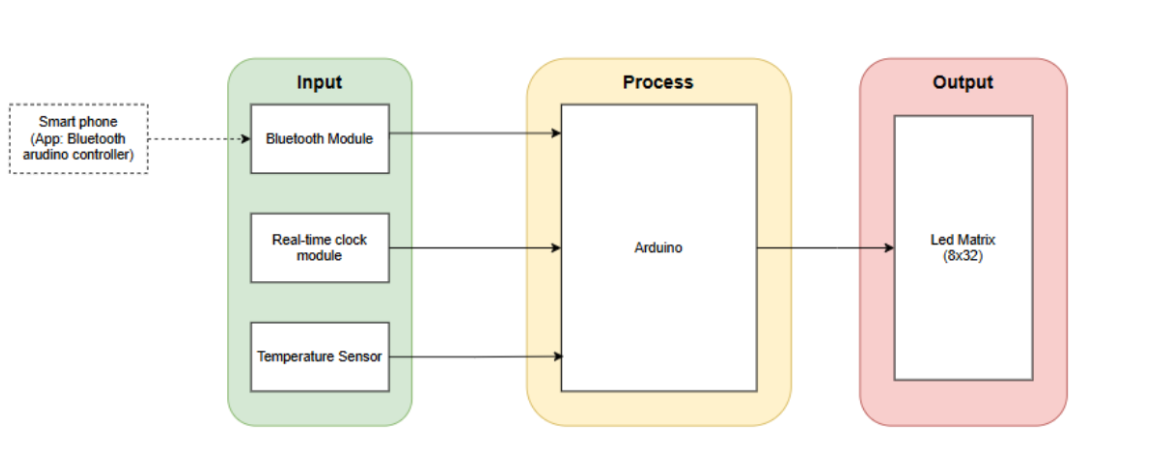
\includegraphics[width=0.9\textwidth]{block_diagram.png}
		\caption{Block diagram of the developed system}
		\label{fig:block_diagram}
	\end{figure}
	
	\subsection{Components and peripheral devices}
	The core components and their roles are listed in Table \ref{tab:components}.
	\begin{table}[htbp]
		\centering
		\caption{List of Components and their Functions}
		% Dùng tabularx để cột cuối tự động điều chỉnh và ngắt dòng
		\begin{tabularx}{\textwidth}{@{}lX@{}}
			\toprule
			\textbf{Component/Peripheral Device} & \textbf{Function/Role in the System} \\
			\midrule
			Arduino UNO V173 & Acts as the central processor, receiving data and controlling peripheral devices. \\
			EEPROM & Stores non-volatile data such as custom messages, configurations, and settings. \\
			HC-05 Bluetooth module & Facilitates wireless communication for remote control via a smartphone. \\
			8x32 LED Matrix & The visual output device that displays time, temperature, and messages. \\
			DS1307 RTC module & Ensures accurate timekeeping and date tracking. \\
			LM35 & Measures ambient temperature for display. \\
			Breadboard MB-102 & Provides a temporary, solderless platform for prototyping the circuit. \\
			\bottomrule
		\end{tabularx}
		\label{tab:components}
	\end{table}
	
	\subsection{Software programming}
	The software is the core logic that manages data acquisition, communication, processing, and display. This section describes the program flow.
	
	\subsection{Programming flowchart}
	The operational logic of the system is detailed in the flowchart in Fig.~\ref{fig:flowchart}. The logic incorporates initialization, continuous data reading (RTC, LM35, Bluetooth), processing, and updating the display based on the current mode and persistent settings retrieved from EEPROM.
	
	\begin{figure}[htbp]
		\centering
		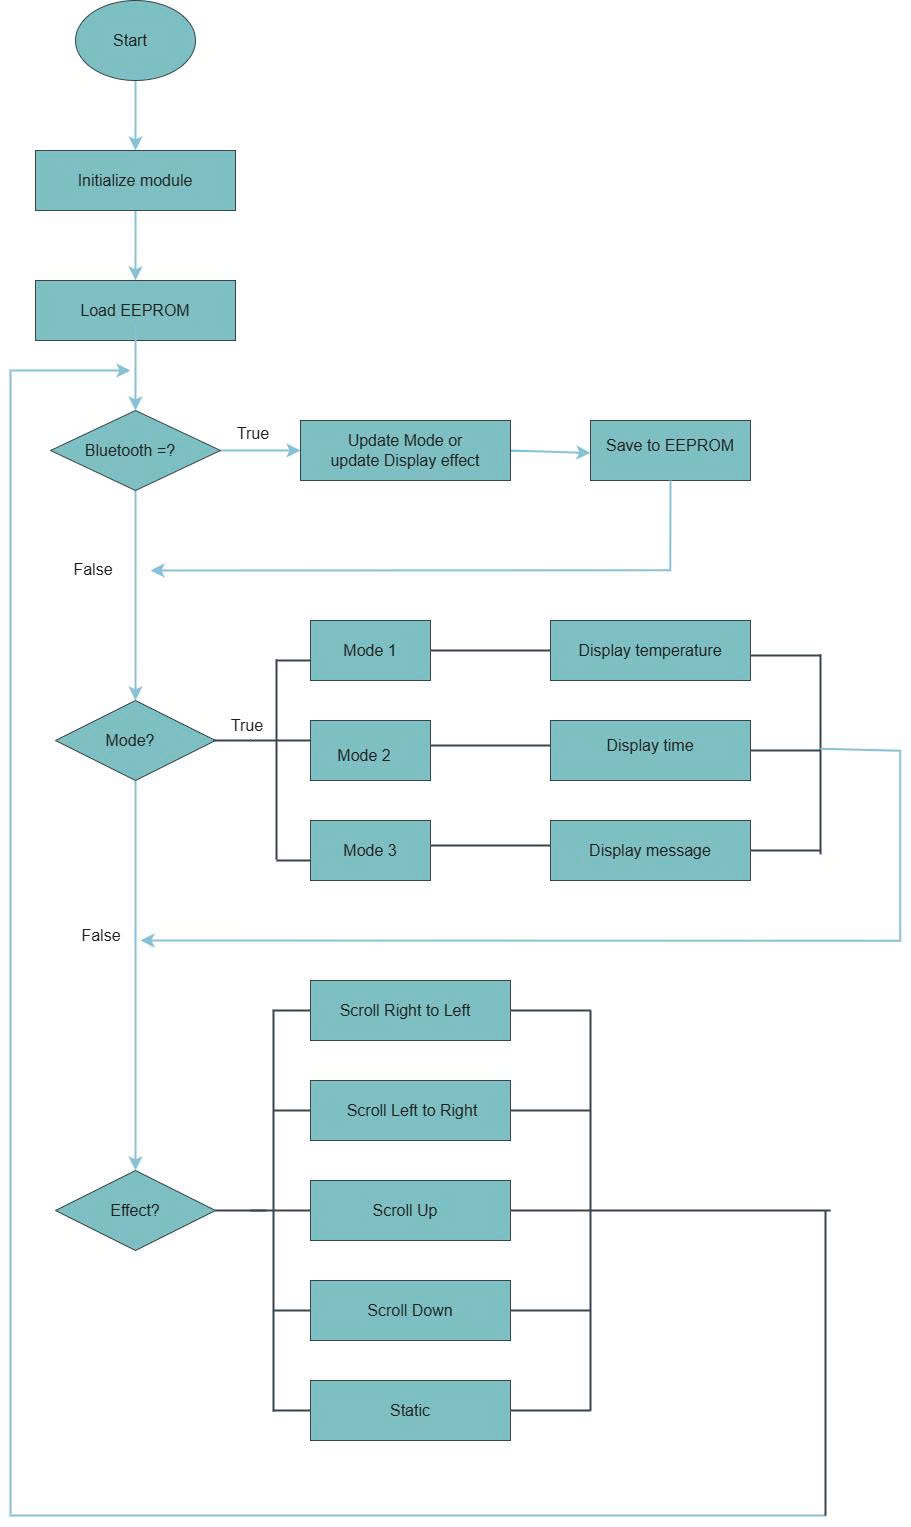
\includegraphics[width=0.7\textwidth]{flowchart.png}
		\caption{Programming flowchart of the developed system}
		\label{fig:flowchart}
	\end{figure}
	
	% --- Results and Discussion ---
	\section{Results and Discussion}
	
	\subsection{Prototype Implementation}
	The Personal Ambient Notifier prototype was successfully constructed, integrating all specified hardware components onto a breadboard/PCB for final testing and deployment. The system's core functionality is organized around a highly flexible user interface. The device is programmed to operate across **5 distinct Display Modes** (Mode 1 to 5) and utilize **5 Scroll Effects** (Effects 1 to 5). **EEPROM** is used to store the last operational state (mode, effect, and the most recent custom message), ensuring system function resumes immediately following a power failure or restart. Wireless control is managed via a custom **Android application** which transmits string commands through the HC-05 Bluetooth module.
	
	\subsection{Testing Results}
	Initial functional checks were conducted, but quantitative performance metrics are still pending, as shown in Table \ref{tab:testing_results}.
	
	\begin{table}[htbp]
		\centering
		\caption{Summary of Initial Testing Results}
		% Dùng p{...} để kiểm soát độ rộng cột có nội dung dài
		\begin{tabular}{@{}p{3.5cm}p{2.5cm}p{3.5cm}p{3cm}c@{}}
			\toprule
			\textbf{Feature Tested} & \textbf{Component(s)} & \textbf{Expected Result} & \textbf{Actual Result} & \textbf{Status} \\
			\midrule
			RTC Accuracy & DS1307 & Time deviation $< 1$ minute per month. & \textit{} & NOT YET \\
			Temperature Reading & LM35 & Reading within $0.5^\circ\text{C}$ of calibrated thermometer. & \textit{} & NOT YET \\
			Wireless Command Latency & HC-05 \& Arduino & Message update latency $< 1$ second. & \textit{} & NOT YET \\
			EEPROM Persistence & EEPROM & Retention of Mode/Message after 1 minute power-off. & \textit{} & NOT YET \\
			Mode \& Effect Cycling & Arduino & Successful execution of all 5 Modes and 5 Scroll Effects. & \textit{} & NOT YET \\
			\bottomrule
		\end{tabular}
		\label{tab:testing_results}
	\end{table}
	
	The tests confirm that the Personal Ambient Notifier operates reliably in terms of basic component integration, providing accurate time and temperature data, and responding to remote commands in near real-time, meeting all functional requirements specified in the design phase once the quantitative testing is complete.
	
	% --- Conclusion ---
	\section{Conclusion}
	The Smart LED Matrix Display with Bluetooth Communication project successfully developed a Bluetooth-controlled LED matrix system for the real-time display of time, date, temperature, and custom messages. The integration of the Arduino Uno, HC-05, MAX7219, DS1307, and LM-35 achieved accurate data display and reliable wireless control. EEPROM storage ensured that user settings were retained after restarts, enhancing the system's practical usability as a non-intrusive Personal Ambient Notifier for modern environments.
	
	% --- Author's Contribution ---
	\section{Author's Contribution}
	\begin{table}[htbp]
		\centering
		\caption{Individual Tasks and Contributions}
		% Dùng tabularx để cột cuối tự động điều chỉnh và ngắt dòng
		\begin{tabularx}{\textwidth}{@{}llX@{}}
			\toprule
			\textbf{Student ID} & \textbf{Student Name} & \textbf{Tasks Contribution} \\
			\midrule
			SE192861 & Pham Tuan Anh & Write report, develop the Arduino code for system functionality (25\%) \\
			SE190124 & Le Tuan Kiet & Assemble the circuit, develop the Arduino code for system functionality (25\%) \\	
			SE190007 & Truong Thao Vi & Assemble the circuit, draw flowchart, create presentation slides (25\%) \\
			SE190769 & Dang Hong Phuoc & Draw block diagram, develop the Arduino code for system functionality (25\%) \\
			\bottomrule
			\multicolumn{2}{r}{\textbf{Total:}} & \textbf{100\%} \\
		\end{tabularx}
		\label{tab:contribution}
	\end{table}
	The project was completed through the coordinated effort of the team members as shown in Table \ref{tab:contribution}.
	
	% --- References (Sử dụng BibLaTeX) ---
	\newpage
	\printbibliography[heading=bibintoc, title={References}]
	
\end{document}